  No planejamento de um sistema energ\'etico hidrot\'ermico o sistema deve preservar as metas de gera\c c\~ao para suprir a demanda e minimizar o valor esperado do custo de
  opera\c c\~ao ao longo do per\'iodo de estudo. Dessa forma, a preserva\c c\~ao da demanda e a minimiza\c c\~ao do valor
  do custo esperado caracterizam o despacho de energia definido no cap\'itulo anterior
  . Diante das possibilidades de configura\c c\~oes poss\'iveis para o sistema (sequ\^encia de acionamento das hidrel\'etricas e das termoel\'etricas com o aumento da demanda para uma produtibilidade fixa) deseja-se obter a combina\c
  c\~ao na qual o valor do custo
  associdado seja m\'inimo. Portanto, o despacho de energia trata-se de um problema de otimiza\c c\~ao. Tal
  problema \'e definido por: dados dois conjuntos 
  $D $ e $\Psi$ subconjuntos do $\mathbb {R}^n$ e uma  fun\c c\~ao $f: \Psi
  \rightarrow R$ o objetivo \'e encontrar um minimizador de $f$ no conjunto $D$ \cite{alexey}. Isto \'e, 
  	\begin{align}%DEFINITION  OF FUNCTION OBJECTIVE 
		\label {obj}
	  	\min_{x\in D} f(x), 
	\end{align}
  define-se o conjunto D como o conjunto vi\'avel do problema, os pontos de D ser\~ao chamados pontos vi\'aveis e $f$ ser\'a chamada
  de fun\c c\~ao objetivo. Uma vez formulado o problema em \eq{obj} para a sua resolu\c c\~ao \'e necess\'ario uma
  defini\c c\~ao dos elementos que constituem um problema do otimiza\c c\~ao. Nesta perspectiva s\~ao abordadas as defini\c c\~oes
  consideradas de relev\^ancia para o presente estudo dadas a seguir.
  	\begin{defin}%DEFINITION OF MINIMIZER  
		\label{def1}
		Um ponto $\bx {x} \in D$ \'e, 
		\begin{enumerate}
			\item minimizador global para \eq{obj} se,
				$$ f(\bx x) \leq f(x), \forall x \in D;$$
			\item minimizador local da \eq{obj}, se existe uma vizinhan\c ca $U$ de \bx {x} tal que
				$$ f(\bx {x})\leq f(x), \forall x \in D \cap U.$$
		\end{enumerate}
	\end{defin}
  \noindent

 Pode-se definir de maneira equivalente o minizador local como,
 	\begin{align}% DEFINITION OF EQUIVALENCE FOR THE MINIMIZER     
		\label{eq2}
		{\bx {x} \in D} & \mbox{ \'e minizador local} \nonumber \\
	 	& \Updownarrow \\
	 	\exists  \epsilon > 0 \enspace \mbox{t.q} \enspace f(\bx {x}) \leq f(x), & \enspace \forall x \in \{ x \in D; ||x -
	   	\bx{x}|| \leq \epsilon \} \nonumber 
  	\end{align}

  Adotando-se $x_g$ e $x_l$ minizador global e local respectivamente o entendimento intuitivo das ideias apresentadas
  \'e dado pela \fig{fig1} a seguir:
  	\begin{figure}[!h]%THE VIABLE WITHOUT RESTRICTIONS 
		\label{fig1}
		\centering
		\resizebox{0.8\width}{!}{
			  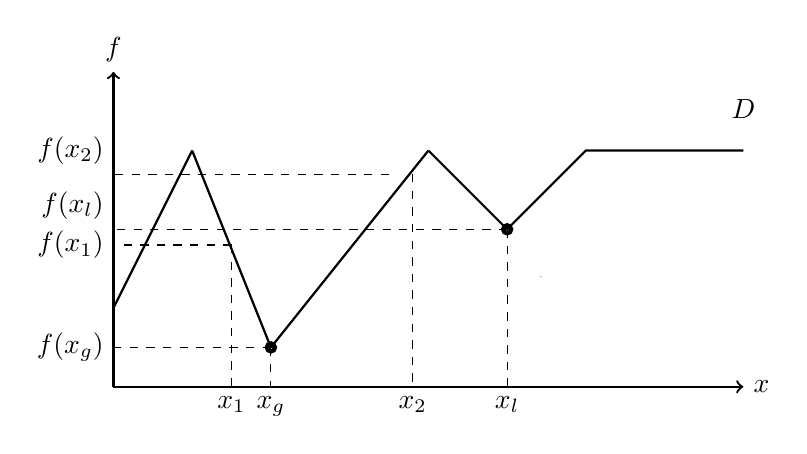
\begin{tikzpicture}
		\draw [->, thick, black] (0,0)--(8,0) node[right] {$x$};
		\draw [->, thick, black] (0,0)--(0,4) node[above] {$f$};
		\draw [thick, black] (0,1)--(1,3);
		\draw [thick, black] (1,3)--(2,0.5); 
		%\draw [thick, black] (1,3)--(2,0.5) node[above,xshift = 3,yshift = 16] {$G$};
		\draw [thick, black](2,0.5)--(4,3);
		\draw [thick, black](4,3)--(5,2); 
		%\draw [thick, black](4,3)--(5,2) node[below left] {$L$};
		\draw [thick, black](5,2)--(6,3)--(8,3)node[above,yshift=8] {$D$};
		%\draw [thick, black](5,2)--(6,3)--(8,3)node[above,yshift=8] {$D$};
		\draw [ultra thick, black](2,0.5) circle (0.5mm);
		\draw [ultra thick, black](5,2) circle (0.5mm);
		\draw [dashed, black](2,0.5)--(0,0.5) node[left] {$f(x_g)$} ;
		\draw [dashed, black](2,0.5)--(2,0) node[below] {$x_g$};
		\draw [dashed, black] (1.5,1.8)--(1.5,0) node[below] {$x_1$};
		\draw [dashed, black] (1.5,1.8)--(0.0,1.8) node[left] {$f(x_1)$};
		\draw [dashed, black](3.8,2.7)--(3.8,0) node[below] {$x_2$};
		\draw [dashed, black](3.5,2.7)--(0.0,2.7) node[above left] {$f(x_2)$};
		\draw [dashed, black](5,2)--(0,2) node[above left] {$f(x_l)$};
		\draw [dashed, black](5,2)--(5,0) node[below] {$x_l$};
		\draw [dashed, black](5,0)--(5,2);
	%	\draw [dashed, black](5,0)--(5,2) node[above, yshift = 8] {$U$};
		%\draw [thin, black] (5,2)--(5.7,1)[above left];
		\draw [very thin, black] (5.43,1.4) circle (0.01mm);  
		%\draw [very thin, black] (5.43,1.4) circle (0.01mm) node[above] {$\epsilon$};  
		%\draw [thin, black](5,2) circle (12.0mm); 
	  \end{tikzpicture}
 
  	}
		\caption{Minizador global ($x_g$), local ($x_l$) e vizinhan\c ca (U).}
  	\end{figure}

  Observando-se a \fig{fig1} percebe-se  que um minimizador local existe quando \'e poss\'ivel
  encontrar uma regi\~ao $\mathrm{U}$ em $\mathrm{D}$ na qual seja satisfeita a rela\c c\~ao $f(\bx{x}) \leq f(x)$.
  Nota-se pela \df{def1} que um minizador global tamb\'em \'e um minizador local, contudo a rec\'iproca n\~ao 
  \'e verdadeira \cite{alexey}. O fato do minizador local necessitar de apenas uma vizinha\c ca $U$ em $D$  indica a possibilidade da fun\c
  c\~ao $f$ ter 
  v\'arios minizadores locais no conjunto vi\'avel D. \'E importante salientar que dependendo do problema de otimiza\c
  c\~ao pode existir restri\c c\~oes no conjunto vi\'avel $D$. Portanto, considerando-se o problema,
  	\begin{align}%PROBLEM WITH RESTRICIONS  
		\min_{x,x_d \in D; x \geq x_d} f(x)
		\label{eq3}
	\end{align}
  a situa\c c\~ao \'e exemplificada em \fig{fig11}.
  	\begin{figure}[!htpb]%THE SET VIABLE WITH RESTRICTIONS
		\centering
		\resizebox{0.8\width}{!}{
			  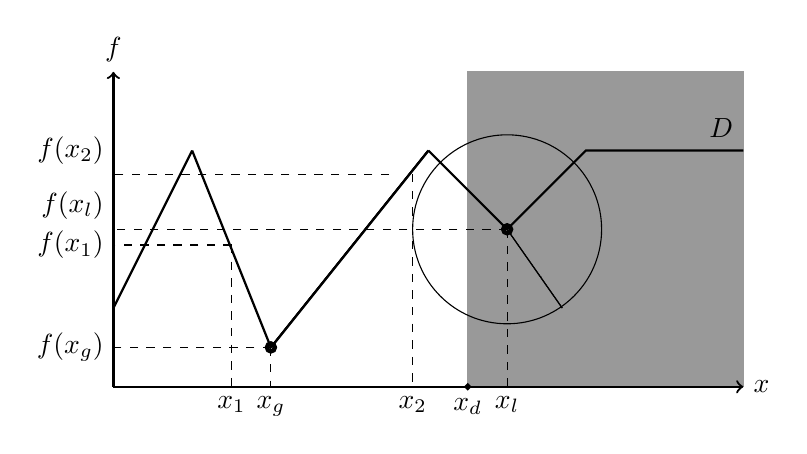
\begin{tikzpicture}
  \draw [->, thick, black] (0,0)--(8,0) node[right] {$x$};
  \draw [->, thick, black] (0,0)--(0,4) node[above] {$f$};
  \draw [thick, black] (0,1)--(1,3);
  \draw [thick, black] (1,3)--(2,0.5); 
  %\draw [thick, black] (1,3)--(2,0.5) node[above,xshift = 3,yshift = 16] {$G$};
  \draw [thick, black](2,0.5)--(4,3);
  \draw [thick, black](2,0.5)--(4,3);
  \draw [thick, black](4,3)--(5,2) ;
  %\draw [thick, black](4,3)--(5,2) node[below left] {$L$};
  \draw [thick, black](5,2)--(6,3)--(8,3)node[left,yshift=8] {$D$};
  \draw [ultra thick, black](2,0.5) circle (0.5mm);
  \draw [ultra thick, black](4.5,0) circle (0.1mm) node[below]{$x_d$};
  \draw [dashed, black](5,2)--(5,0) node[below] {$x_l$};
  \draw [ultra thick, black](5,2) circle (0.5mm);
  \fill [black, draw=black, opacity = 0.4] (4.5,0) rectangle (8,4);
  \draw [dashed, black](2,0.5)--(0,0.5) node[left] {$f(x_g)$};
  \draw [dashed, black](2,0.5)--(2,0) node[below] {$x_g$};
  \draw [dashed, black] (1.5,1.8)--(1.5,0) node[below] {$x_1$};
  \draw [dashed, black] (1.5,1.8)--(0.0,1.8) node[left] {$f(x_1)$};
  \draw [dashed, black](3.8,2.7)--(3.8,0) node[below] {$x_2$};
  \draw [dashed, black](3.5,2.7)--(0.0,2.7) node[above left] {$f(x_2)$};
  \draw [dashed, black](5,2)--(0,2) node[above left] {$f(x_l)$};
  \draw [very thin, black] (5.43,1.4) circle (0.01mm);  
  %\draw [very thin, black] (5.43,1.4) circle (0.01mm) node[above] {$\epsilon$};  
  \draw [thin, black] (5,2)--(5.7,1)[above left];
  \draw [dashed, black](5,0)--(5,2);
  %\draw [dashed, black](5,0)--(5,2) node[above, yshift = 8] {$U$};
  \draw [thin, black] (5,2)--(5.7,1)[above left];
  \draw [thin, black](5,2) circle (12.0mm); 
  \end{tikzpicture}

	}
		\caption{M\'inimo global ($x_g$), local ($x_l$) e conjunto com restri\c c\~oes D.}
  		\label{fig11}
	\end{figure}
	\newpage
De acordo com \fig{fig11} apesar de $x_g$ ser o m\'inimo de $f$ a restri\c c\~ao $ x\geq x_d$ torna invi\'avel $x_g$
ser o minizador para a fun\c c\~ao $f$ considerando-se o conjunto vi\'avel $D$, portanto, neste caso o minizador
corresponde ao elemento $x_l$.\\
  Considerando-se o problema de minimiza\c c\~ao na \eq{obj} o valor \'otimo \'e 
  o menor valor que $f(x)$ assumir considerando-se $x \in D$ essa ideia embasar a \df{def2}. 
  	\begin{defin}
		\label{def2}
		Seja $\bx {v} \in [-\infty, +\infty)$ definido por,
	  	\begin{equation*}
			\bx {v} =  \underset{x \in D} {\textrm{inf}} \ \ f(x)
	  	\end{equation*}
	  	\bx {v} \'e o valor \'otimo da \eq{obj}.
	\end{defin}
Nota-se pela \df{def2} que o objeto a ser encontrado (valor \'otimo) est\'a bem definido. O fato de tomar o inf indica
que o valor \'otimo pode n\~ao pertence ao conjunto de restri\c c\~oes $D$, contudo deve est\'a suficiente pr\'oximo
para ser considerado de relev\^ancia para n\~ao comprometer a solu\c c\~ao do problema dado pela \ref{obj}. 
De forma geral problemas de minimiza\c c\~ao est\~ao relacionados com problemas de maximiza\c c\~ao. De fato, uma rela\c c\~ao bastante 
conhecida entre problemas de maximiza\c c\~ao e minimiza\c c\~ao \'e encontrada em \cite{alexey} dada por,
	\begin{align}
  		\label{eq4}
		\max_{x \in D} f(x) \Leftrightarrow  
		\min_{x \in D} -f(x).
  	\end{align}
Desta forma, problemas de minimiza\c c\~ao e maximiza\c c\~ao podem ser interpretados como o mesmo tipo de
problema, entretanto as solu\c c\~oes locais e globais do problema \ref{eq4} evidentemente possuem sinais opostos. A
exemplifica\c c\~ao deste fato \'e dada pela \fig{fig2}.
	\begin{figure}[!htpb]%MINIMIZER AND MAXIMIZER 
		\centering
		\resizebox{0.5\textwidth}{!}{
			\begin{tikzpicture}
  \draw [blue, thick, domain=-2:2] plot(\x,{1 +\x*\x}) node[below right, thick, black,xshift=8.0] {$-f$};
  \draw [very thin, black, dashed] (0,1)--(0,0) node[below right] {$\bx{x}$};    
  \draw [very thin, black, dashed] (0,0)--(0,-1);    
  \draw [red, thick, domain=-2:2] plot(\x,{-1 -\x*\x}) node[above right,thick, black,xshift=8.0] {$f$};
  \draw [thick, black,->] (-5,0)--(5,0); 
  \draw [thick, black,->] (-3,-5)--(-3,5);
  \draw [thick, black, dashed] (0,1)--(-3,1) node[left] {$-\bx{v}$};
  \draw [thick, black, dashed] (0,-1)--(-3,-1) node[left] {$\bx{v}$};
\end{tikzpicture}

		}  \caption{Minimiza\c c\~ao ($-f$) e Maximiza\c c\~ao ($f$).}
		\label{fig2}
	\end{figure}

O conjunto vi\'avel de um problema de 
otimiza\c c\~ao \'e definido por um conjunto de igualdades e/ou desigualdades e/ou inclus\~ao da seguinte forma,
	\begin{equation*}%THE SET VIABLE
  		D = \left \{ x \in \Psi; \begin{array}{cc} h_i(x) = 0, i = 1, \dots, l \\ g_j(x) \leq 0, j = 1, \dots, m  \end{array} \right \}
	\end{equation*}
ou de forma equivalente, 
	\begin{equation*}%DEFINITION FOR SET VIABLE
  		D = \{ x \in \Psi; h(x) = 0, g(x) \leq 0\}.
	\end{equation*}
dado que $\Psi \subset \mathbb{R}^n$, $h:\Psi \rightarrow R^l$ e $g: \Psi \rightarrow \mathbb{R}^{m}$ admitindo-se que $f$ est\'a 
definida no conjunto $\Psi$. O conjunto  $\Psi$ representa as condi\c c\~oes diretas e as desigualdades 
s\~ao conhecidas como restri\c c\~oes funcionais. Na pr\'atica, a separa\c c\~ao entre restri\c c\~oes diretas e funcionais \'e apenas 
uma conveni\^encia. De fato, seja a condi\c c\~ao direta $x \in \Psi = \mathbb{R}_+^n$ \'e equivalente a
representa\c c\~ao funcional dada por  $x \in \{x \in R^n; x_i \geq 0, i = 1,\dots, n \}$ \cite{alexey}. No conjunto de restri\c
c\~oes $D$ em alguns casos existe a necessidade de manipula\c c\~oes e/ou transforma\c c\~oes para tornar poss\'ivel ou facilitar a resolu\c
c\~ao do problema de otimiza\c c\~ao. 
Por exemplo, as restri\c c\~oes de igualdade $h_i = 0$ podem ser reescritas de maneira equivalente como inequa\c c\~oes, ou seja, 

	\begin{align*}%EQUIVALENT WRITING OF THE EQUALITY RESTRICTION
		h_{i} (x) & = 0 \\
		& \Updownarrow \hspace{1.4cm} \mbox{com $i = 0,1, \dots, l$}\\ 
		h_{i} \leq 0,& -h_{i}(x) \leq 0. 
	\end{align*}

De forma, an\'aloga pode-se transformar restri\c c\~oes de desigualdade mediante uma transforma\c c\~ao inserindo nas inequa\c c\~oes
termos artificiais conhecidos como vari\'aveis de folga, isto \'e, 
	\begin{align*}%VARIABLE OF BACKSLASH
		g_{i} (x) & \leq 0 \\ 
 		&\Updownarrow \hspace{1.4cm} \mbox{com $i = 0,1, \dots, l$}\\ 
 		g_{i}  + z_i^2 & = 0, z_i \in R. 
	\end{align*}

Contudo, na pr\'atica dependendo do contexto o problema de otimiza\c c\~ao pode-se tornar mais complexo com tais transforma\c c\~oes 
sua utiliza\c c\~ao dever ocorrer quando realmente existe alguma indica\c c\~ao do melhoramento do problema transformado em compara\c c\~ao com o
problema original. Em
primeiro lugar existe a possibilidade do problema relaxado possuir condi\c c\~oes de otimalidade mais fracas que o problema com as 
restri\c c\~oes originais \cite{alexey}. Outro fator a ser considerado \'e 
o aumento no n\'umero de restri\c c\~oes. Quanto ao tipo de problema em rela\c c\~ao ao conjunto de restri\c c\~oes ($D$),
por enquanto deve-se considerar basicamente dois casos especificos: sem restri\c c\~oes quando $D = R^n$, isto \'e, sem
restri\c c\~oes no dom\'inio no qual $f$ \'e definida. Uma exemplifica\c c\~ao deste caso pode ser observado na \fig{fig1}.
Para o caso $D \neq R^n$ tem-se um problema com restri\c c\~oes, ou seja, deve-se considerar um subconjunto do
dom\'inio de $f$ um exemplo \'e dado na \fig{fig11}. O conjunto das restri\c c\~oes \'e de 
fundamental import\^ancia para o estudo da otimiza\c c\~ao \cite{alexey}. De fato, uma classe importante de problemas \'e definida quando
o conjunto das restri\c c\~oes 
forma um poliedro.
	\begin{defin}%DEFINITION OF THE POLYHEDRAL SET
  		Um conjunto \'e dito poliedral quando ele pode ser representado como um conjunto de solu\c c\~oes de um sistema finito de equa\c c\~oes 
  		e inequa\c c\~oes lineares, isto \'e,
		\begin{equation*}%VIABLE SET
  			D = \left\{ x \in R^n; Ax = a, Bx \leq b \right\},
		\end{equation*}
		onde:
		\begin{itemize}
			\item $R(l,n)$ \'e um elemento do espa\c co de matrizes de $l$ linhas por $n$ colunas;
			\item $R(m,n)$ \'e um elemento do espa\c co de matrizes de $m$ linhas por $n$ colunas;
			\item $A \in R(l,n)$, $B \in R(m,n)$;
			\item $a \in R^l$ e $b \in R^m$.
		\end{itemize}
		\begin{figure}[!h]%POLYHEDRAL SET
			\centering
			\label{pol} 
			\resizebox{2.5\width}{!}{
			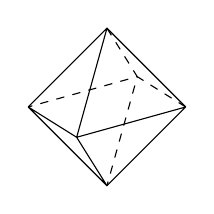
\begin{tikzpicture}
	\path
	( 1, 0, 0) coordinate (A1)
	( 0, 0,-1) coordinate (A2)
	(-1, 0, 0) coordinate (A3)
	( 0, 0, 1) coordinate (A4)
	( 0, 1, 0) coordinate (B1)
	( 0,-1, 0) coordinate (B2);

	\draw 
	(A1)--(A4)--(A3)
	(B1)--(A4)--(B2)
	(A1)--(B1)--(A3)
	(A1)--(B2)--(A3);

	\draw[dashed]
	(A1)--(A2)--(A3)
	(B1)--(A2)--(B2);
\end{tikzpicture}

			}
			\caption{Exemplo de um conjunto poliedral  $\mathbb{R}^3$.}
		\end{figure}
	\end{defin}
	Desta forma tomando-se $h:R^n \rightarrow R^l$ e $g: R^n \rightarrow R^m$ definidas como $h(x) = Ax -a$ e $g(x) = Bx -
b$ fun\c c\~oes afins nesse contexto \cite{alexey}. Nota-se que para o caso do $\mathbb{R}^{2}$ teriamos um
pol\'igono no plano.  
Uma vez que o conjunto poliedral est\'a bem definido pode-se estabelecer informa\c c\~oes \'uteis sobre a fun\c c\~ao
objetivo $f$. 
	\begin{defin}%DEFINITION OF THE FUNCTION PUADRATIC
  		Uma fun\c c\~ao $f: R^n  \rightarrow R$, definida por,
  		$$ f(x) = \left < Px,x \right > + \left < q, x \right > $$
  		onde $P \in R(n,n),q \in R^n$, \'e chamada fun\c c\~ao quadr\'atrica.
  		\label{fun}
	\end{defin}
Dada P em \autoref {fun} pode-se admitir sem perca de generalidade que est\'a \'e sim\'etrica, portanto,
	\begin{equation*}%RELATION OF THE FUNCTION PUADRATIC
  		\left <Px,x \right > = \frac {1} {2} \left < (P + P^T)x, x \right >.
	\end{equation*}
Uma vez que \'e poss\'ivel a substitui\c c\~ao da matriz P pela sim\'etrica $ \frac{(P + P^t)} {2}$ \cite{alexey}.
Desta forma considera-se dois casos
de grande import\^ancia: o conjunto ($D$) \'e poliedral e a fun\c c\~ao ($f$) \'e quadr\'atrica trata-se de um problema de programa\c
c\~ao quadr\'atrico para o caso que o conjunto ($D$) \'e poliedral  e a fun\c c\~ao objetivo ($f$) seja linear,
ou seja, quando $P = 0$ em \autoref{fun} trata-se de um problema de programa\c c\~ao linear. Para o presente trabalho
ser\'a considerado somente problemas de programa\c c\~ao linear. Contudo, somente a informa\c c\~ao sobre o conjunto $D$
ser um conjunto poliedral n\~ao permite considera\c c\~oes que facilite a buscar pela a solu\c c\~ao do problema liner,
al\'em de n\~ao permitir verificar se a solu\c c\~ao encontrada \'e realmente adequada para o problema proposto na 
\eq{obj}. Com esse intuito ser\'ao tratado somente os aspectos de
relev\^ancia da an\'alise convexa para o tratamento adequado do conjunto poliedral ($D$) e para o desenvolvimento de
outros resultados importantes para o presente estudo.  
 	\begin{defin}%DEFINITION OF THE CONVEX SET
	 	\label{conv}
	 	Um conjunto  $Q \subset R^n$ \'e chamado conjunto convexo se para quaisquer $x \in Q$, $y \in Q$ e $\forall \lambda \in [0,1]$ tem-se que 
     	$\lambda x + (1 - \lambda)y \in Q$.
     	Onde tem-se que o ponto $\lambda x + (1 - \lambda)y$ \'e uma combina\c c\~ao convexa de $x$ e $y$ com o par\^ametro
     	$\lambda$.
 	\end{defin}
 \noindent
 Dada a defini\c c\~ao \autoref{conv} para que um conjunto $Q$ qualquer seja convexo \'e necess\'ario que dados dois
 pontos de $Q$ o segmento de reta cujos os extremos sejam esses pontos deve est\'a no conjunto $Q$.
 	\begin{defin}%DEFINITION OF THE CONVEX FUNCTION 
		\label{conv2}
   		Se $Q \subset R^n$ \'e um conjunto convexo, diz-se que a fun\c c\~ao $f:Q \rightarrow R$ \'e convexa em $Q$ quando para quaisquer 
    	$x \in Q$, $y \in Q$ e $\lambda \in [0,1]$ tem-se que,
   			\begin{equation*}
	    		f(\lambda x + (1-\lambda)y) \leq \lambda f(x) + (1-\lambda)f(y).
   			\end{equation*}
	\end{defin}
 \noindent
 As defini\c c\~oes \autoref{conv} e \autoref{conv2} caracterizam os elementos principais de convexidade. Por meio da
 convexidade \'e poss\'ivel determinar caracter\'isticas favor\'aveis na resolu\c c\~ao da \eq{obj}. Por exemplo, os
 resultados a seguir permitem descrever os objetos que formam o conjunto vi\'avel (D) como conjuntos convexos.
 	%RESULTS FOR CONVEXITY
 	\begin{prop}%ALL SEMI-SPACE IN R^N IS CONVEX
	 	\label{propv1}
	 	Qualquer semi-espa\c co em $\mathbb{R}^n$, isto \'e, o conjunto da forma $D = \{x \in R^n;\left <x,a \right >  \leq
	 	c\}$ onde $a \in R^n$ $c \in R$ \'e convexo.\\
	 	Prova: 
	 	De fato, tomando-se $x,y \in D$ e definindo uma $f: D\rightarrow R$ tal que,
	 		\begin{align*}
		 		f(x) =\left <x,a \right >  = \sum_{i = 1}^{n}x_ia_i \hspace{2pt} \mbox{com $x,a \in D$, onde a \'e fixo e $i = 1,2 \dots n$}.
	 		\end{align*}
	 	Portanto, da hip\'otese tem-se que \\
	 		\begin{align}
		 		\left <x,a\right > = \sum_{i = 1}^{n} x_ia_i \leq c \label{eqp1}\\
		 		\left <y,a\right > = \sum_{i = 1}^{n} x_ia_i \leq c  \label{eqp2}.
	 		\end{align}
	 	Tomando $\alpha \in [0,1]$ e multiplicando \ref{eqp1} por ($\alpha$) e \ref{eqp2} por ($1 - \alpha$) tem-se,
	 		\begin{align}
		 		\left <\alpha x,a\right > &= \alpha \sum_{i = 1}^{n} x_ia_i \leq \alpha c \label{eqp1a}\\
		 		\left <\alpha y,a\right > &= (1-\alpha)\sum_{i = 1}^{n} y_ia_i \leq (1 - \alpha)c  \label{eqp2b}.
	 		\end{align}
	 	Somando-se \ref{eqp1a} com \ref{eqp2b} segue que
	 		\begin{align*}
		 		\left <\alpha x,a\right > + \left <(1-\alpha) y,a\right >  &= \alpha \sum_{i = 1}^{n} x_ia_i + (1-\alpha)\sum_{i =
		 		0}^{n} y_ia_i \leq \alpha c + (1 - \alpha)c \Rightarrow \nonumber\\
		 		\left <\alpha x,a\right > + \left <(1 -\alpha) y,a\right >  &= \alpha f(x) + (1 - \alpha)f(y) \leq c
	 		\end{align*}
	 	pela defini\c c\~ao \autoref{conv} a prova est\'a terminada.
	\end{prop}
	\begin{prop}%ALL SEMI-FLAT IN r^N IS CONVEX
		\label{propv2}
		Qualquer hiperplano em $\mathbb{R}^n$, isto \'e, o conjunto da forma $D = \{x \in R^n;\left <x,a \right >  \leq
	 	c\}$ onde $a \in R^n$ $c \in R$ \'e convexo. \\
	 	Prova:\\
	 	De maneira an\'aloga a proposi\c c\~ao \autoref{propv1} deve-se utilizar "$=$" ao inv\'es de "$\leq$".
	\end{prop}
	\begin{prop}%INTERSECTION OF THE CONVEX SETS IS CONVEX 
		\label{proconv}
 		Sejam $D_i \subset \mathbb R^n$, tal que $i \in I$, conjuntos convexos onde I \'e um conjunto qualquer (possivelmente infinito). \\
  		Ent\~ao a intersec\c c\~ao $D = \cap _{i \in I} D_i$ tamb\'em \'e um conjunto convexo \cite{alexey}.
 	\end{prop}
	\begin{cor}%THE CONVEX SET IN R^N IS CONVEX 
		\label{cov1}
		Um conjunto poliedral em $\mathbb{R}^n$ \'e convexo \cite{alexey}.\\
		Prova:

		De fato, o conjunto vi\'avel de \eq{obj} \'e um poliedro formado pela intersec\c c\~ao de semi-espa\c cos e
		hiperplanos nota-se pelas preposi\c c\~oes \autoref{propv1} e \autoref{propv2} que tais conjuntos s\~ao convexos, logo,
		segue pela proposi\c c\~ao \autoref{proconv} que conjunto ($D$) \'e convexo.
	\end{cor}
 \noindent

  Dessa forma, o  conjunto de problemas de otimiza\c c\~ao quadr\'atricos
 e lineares com o conjunto ($D$) de restri\c c\~oes podem sem perca de generalidade serem tratados como conjuntos
 convexos, portanto, quando houver refer\^encia ao conjunto vi\'avel ($D$) ser\'a considerado tanto como um conjunto poliedral
 como tamb\'em um conjunto convexo. 
 A proposi\c c\~ao \autoref{proconv} e o corol\'ario \autoref{cov1} podem ser encontrados com maiores detalhes em \cite{alexey}. 
 O fato de se poder trabalhar com o conjunto 
 das restri\c c\~oes de um problema de otimiza\c c\~ao como um conjunto convexo deve-se ao Teorema de Maximiza\c c\~ao de uma fun\c c\~ao 
 convexa em um conjunto poliedral. Diretamente deste teorema obt\'em-se uma forma de assegurar a 
 exist\^encia de uma solu\c c\~ao para um problema de programa\c c\~ao linear. Al\'em de indicar uma formula\c c\~ao
 para a buscar da  solu\c c\~ao. 
  	\begin{teo}%SOLUTION OF THE PROBLEM IN THE CONVEX SET IS VERTICE OF THE CONVEX SET	
	 	\label{proconv2}
	 	Sejam $D \subset \mathbb{R}^n$ um conjunto poliedral que n\~ao cont\'em nenhuma reta e $f: D \rightarrow R$ uma
	 	fun\c c\~ao convexa. Supondo-se que o problema dado por
	 		\begin{align}
		 		\label{max}
		 		\max_{x \in D} f(x) 
	 		\end{align}
	 	possua uma solu\c c\~ao.
	 	Ent\~ao existe uma solu\c c\~ao deste problema que \'e um v\'ertice de D \cite{alexey}.
 	\end{teo}
 Conforme o teorema \autoref{proconv2} desde que as suposi\c c\~oes sejam respeitadas tem-se uma maneira de encontrar uma
 solu\c c\~ao para o problema \ref{max}. Nota-se que o problema tem caracter\'isticas que se assemelham ao problema
 original dado por \ref{obj}. Contudo, a forma apresentada no teorema \autoref{proconv2} ainda n\~ao \'e a procurada. O
 resultado do corol\'ario \autoref{cov2} estabele a rela\c c\~ao final que o problema esteja bem definido, al\'em de
 permitir um melhor an\'alise do problema proposto por \ref{obj}.
 	\begin{cor}%SOLUTION OF PROBLEM LINEAR IS A VERTICE OF THE VIABLE SET, USE LABEL COV2
	 	\label{cov2}
		Supondo-se que $D \subset R^n$ seja um conjunto poliedral que n\~ao cont\'em nenhuma reta, e que o problema de programa\c c\~ao 
		linear
	   \begin{align} 
		   \label {obj2}
		   \min \left<c,x\right> \mbox{sujeito a} \hspace{6pt}x \in D
	   \end{align}
	    tenha uma solu\c c\~ao, assumindo-se $c \in R^n$. Ent\~ao, um dos v\'ertices de $D$ \'e uma solu\c c\~ao do
		problema. Em particular, quando a solu\c c\~ao \'e \'unica, ela \'e um v\'ertice de $D$ \cite{alexey}.\\
   	   Demonstra\c c\~ao:\\
       De fato, aplicando a rela\c c\~ao entre problemas de maximiza\c c\~ao e minimiza\c c\~ao abordada em \ref{eq4} o problema
	   \ref{obj2} \'e reescrito como,
       \begin{align*}
	   		-\max\left <-c,x \right > \mbox{sujeito a} \hspace{5pt}x \in D.
   		\end{align*}
   		a fun\c c\~ao objetivo desse problema \'e convexa, portanto, o resultado segue da aplica\c c\~ao do
   		teorema \autoref{proconv2}.  
	 Para que que as condi\c c\~oes do teorema sejam satisfeitas \'e necess\'aria uma restri\c c\~ao no conjunto
	 vi\'avel $D$, portanto, tomando $x \geq 0$ garante que o conjunto vi\'avel $D$ n\~ao possui nenhuma reta o que
	 permite que seja poss\'ivel utilizar o resultado.
    \end{cor}
Em problemas de natureza  pr\'atica \'e comum que a vari\'avel de interesse $x$ assume valores n\~ao
negativos, consequentemente a restri\c c\~ao $x \geq 0$ n\~ao se torna um empecilho para a maioria das aplica\c c\~oes.
Por exemplo, considerando-se que uma determinada empresa entregar tr\^es tipos de mercadoria A, B e C. Cada mercadoria
tem um custo $c_1, c_2 \hspace{4pt} \text{e} \hspace{4pt}c_3$ associdado que depende do tempo de entrega 
$t_1,t_2 \hspace{4pt} \text{e} \hspace{4pt}t_3$ respectivamente. Considerando-se que  o custo total possui uma rela\c
c\~ao com o tempo de tal forma que quanto menor o tempo de entregar menor custo associado. Contudo, deve-se garantir a
integridade de cada mercadoria com base em caracter\'isticas espec\'ificas. Portanto, este tipo de
problema poderia ser modelado como,
	\begin{align*}
		\min_{x \in D}\left < c,t \right >
	\end{align*}
onde:
	\begin{itemize}
		\item c \'e o vetor custo;
		\item t \'e o vetor tempo;
		\item D conjunto vi\'avel com as restri\c c\~oes de qualidade.
	\end{itemize}
Nota-se que nesse tipo de situa\c c\~ao n\~ao h\'a um sentido para que a vari\'avel de interesse $t$ seja considerada
negativa.
Desta forma, para a utiliza\c c\~ao do resultado do corol\'ario \autoref{cov2}
tem-se o conjunto vi\'avel $D$ dado por,
	\begin{equation*}%VIABLE CONVEX SET
		D = \left\{ x \in R_+^n; Ax = a, Bx \leq b \right\}.
  	\end{equation*}

Observa-se que o resultado apresentado pelo corol\'ario \autoref{cov2} n\~ao garante que o conjunto $D$ seja limitado. 
Portanto, h\'a a possibilidade que o conjunto vi\'avel do problema de programa\c c\~ao linear n\~ao seja limitado. Nesse
caso  pode ocorrer problemas quanto a buscar pela solu\c c\~ao. A resolu\c c\~ao de um problema de programa\c c\~ao linear
de maneira direta, ou seja, buscando-se o minizador da fun\c c\~ao objetivo $f$ no conjunto vi\'avel $D$ pode n\~ao ser 
a melhor alternativa a depender do caso.
Nesta perspectiva  \'e constitu\'ido o conceito de dualidade de um problema de programa\c c\~ao linear.
O conceito de dualidade  grosso modo \'e uma forma de transforma\c c\~ao de um problema original em um outro problema.
Ambos os problemas possuem a mesma solu\c c\~ao desde que determinadas caracter\'isticas sejam satisfeitas. A principal
justificativa para a utiliza\c c\~ao do problema auxiliar deve-se ao fato que caso o problema original possua um tratamento complexo
frequentemente o problema auxiliar possui uma menor complexidade. 
	\begin{defin}%Dual of problem
		Considerando-se o seguinte problema de programa\c c\~ao de linear que ser\'a denominado de problema primal,
				\begin{align}
					\label {primal}
					\min \left < c,x \right >  \mbox{sujeito a} \hspace{2pt} x \in D = \{ x \in R^n;Bx \geq b \},
				\end{align}
				onde $b \in R^m$, $c \in R^n$ e $B \in R(m,n)$.\\
				O problema dual de \ref{primal} \'e definido como,
			\begin{center}
				\begin{align}
					\label {dual}
					\max \left<b,\mu \right> \mbox{sujeito a} \hspace{2pt} \mu \in \Delta = \{ \mu \in R_{+}^{m}; B^T\mu \leq c\}
				\end{align}
			\end{center}
  	\end{defin}
Algumas considera\c c\~oes que devem ser tomadas no contexto da dualidade de um problema primal. Primeiramente, o
problema primal \'e constitu\'ido por $n$ vari\'aveis com $m$ restri\c c\~oes, por outro lado para o problema dual
s\~ao $m$ vari\'aveis com  $n$ restri\c c\~oes. A natureza dos resultados para a dualidade n\~ao deve ser modificar 
mesmo que o formato do problema primal seja 
modificado. Contudo, esta afirma\c c\~ao  \'e verdadeira deste que o problema dual esteja definido 
adequadamente. Por fim, o seguinte resultado garante a rela\c c\~ao de equival\^encia entre o problema primal e dual.

	\begin{teo} 
		Dualidade em programa\c c\~ao linear.\cite{alexey}\\
		Para o par de problemas \ref{primal} e \ref{dual} as seguintes tr\^es possibilidades s\~ao poss\'iveis:\\ 
		(1) Ambos os problemas possuem o conjunto vi\'avel vazio, i.e, $D = \emptyset$ e $\Delta = \emptyset$.\\
		(2) A fun\c c\~ao objetivo de um dos problemas \'e limitada (inferiormente para \ref{primal} e superiormente para
		\ref{dual}) no conjunto vi\'avel correspondente n\~ao-v\'azio. Neste caso, o outro problema tem o seu conjunto vi\'avel
		vazio.\\
		(3) A fun\c c\~ao objetivo de um problemas \'e limitada (inferiormente para \ref{primal} e superiormente para
		\ref{dual}) no conjunto vi\'avel correspondente n\~ao-v\'azio. Neste caso, ambos problemas possuem solu\c c\~ao e seus
		valores \'otimos coincidem.
	\end{teo}
A terceira possibilidade indica que caso seja poss\'ivel a solu\c c\~ao do problema primal ou dual o valor \'otimo da
fun\c c\~ao objetivo de ambos os problemas
coincide, ou seja, pode-se resolver o problema primal de forma indireta baseando-se no dual associado. Nesse cap\'itulo
foram abordados os principais aspectos da teoria da otimiza\c c\~ao relevante  para o estudo sobre o problema do
despacho de energia. Desde a defini\c c\~ao do conjunto vi\'avel e as rela\c c\~oes que podem ser estabelecidas, al\'em
dos principais conceitos para a resolu\c c\~ao de problemas de programa\c c\~ao linear como a teoria da
dualidade.
